% ============================================================
% PHẦN 5 (Slide 41--50): Quy trình Render 3D Gaussian Splatting
% và cải tiến FastGS -- Mô hình chi phí & ba đòn bẩy tăng tốc
% ============================================================

% --- Slide 41 ---
\begin{frame}{Vì sao 3DGS gốc chậm?}
\begin{itemize}
    \item Mỗi iteration huấn luyện gồm 4 khâu chính: \textbf{render} (chiếu + rasterize), \textbf{tính loss}, \textbf{backward} (lan truyền ngược), và định kỳ \textbf{densify/prune}.
    \item Với cảnh thực tế có hàng trăm nghìn đến hàng triệu Gaussian, chi phí \textbf{rasterize} và \textbf{backward} chiếm phần lớn thời gian mỗi bước.
    \item Densify/prune chỉ chạy định kỳ (không phải mỗi iteration) nhưng gây đột biến chi phí khi thực thi.
\end{itemize}
\vspace{0.3cm}
\centering
\footnotesize
\begin{tabular}{lcc}
\toprule
\textbf{Khâu} & \textbf{Tần suất} & \textbf{Tỉ trọng thời gian (ước lượng)} \\
\midrule
Render (project + rasterize) & mỗi iteration & \textasciitilde 45\% \\
Backward (gradient) & mỗi iteration & \textasciitilde 35\% \\
Tính loss & mỗi iteration & \textasciitilde 10\% \\
Densify/Prune & định kỳ & \textasciitilde 10\% (đột biến) \\
\bottomrule
\end{tabular}
\end{frame}

% --- Slide 42 ---
\begin{frame}{Định luật Amdahl áp dụng cho 3DGS}
\footnotesize
\begin{columns}[T]
\begin{column}{0.52\textwidth}
\begin{itemize}
    \item Tăng tốc một phần hệ thống chỉ mang lại lợi ích bị giới hạn bởi tỉ trọng thời gian phần đó chiếm trong toàn pipeline.
\end{itemize}
\begin{block}{Công thức Amdahl}
\[
\text{Speedup} = \dfrac{1}{(1-p) + \dfrac{p}{s}}
\]
\footnotesize $p$: tỉ trọng thời gian phần được tối ưu; $s$: hệ số tăng tốc riêng của phần đó.
\end{block}
\begin{itemize}
    \item Rasterize + backward chiếm $p$ lớn nhất $\Rightarrow$ FastGS tập trung tối ưu \textbf{đúng chỗ này}.
    \item Tối ưu phần chiếm $p$ nhỏ (vd.\ tính loss) dù $s$ lớn vẫn cho speedup tổng thể không đáng kể.
\end{itemize}
\end{column}
\begin{column}{0.48\textwidth}
\centering

\includegraphics[width=0.95\linewidth]{ch8_amdahl.png}
\end{column}
\end{columns}
\end{frame}

% --- Slide 43 ---
\begin{frame}{Mô hình chi phí chi tiết của một iteration}
\footnotesize
\begin{columns}[T]
\begin{column}{0.52\textwidth}
\begin{itemize}
    \item Gọi $N$ là số Gaussian hiện có, $T_i$ là số tile mà Gaussian thứ $i$ chạm tới (tile\_touched).
\end{itemize}
\begin{block}{Chi phí rasterize}
\[
C_{\text{rasterize}} \sim O\!\left(\sum_{i=1}^{N} T_i\right) = O(N \times \overline{T})
\]
\footnotesize $\overline{T}$: số tile trung bình mỗi Gaussian chạm.
\end{block}
\begin{itemize}
    \item Chi phí densify/prune: $C_{\text{densify}} \sim O(N)$.
    \item Giảm $N$ (prune tốt hơn) hoặc giảm $\overline{T}$ (box nhỏ hơn) đều giảm trực tiếp chi phí -- cơ sở cho 2 trong 3 đòn bẩy của FastGS.
\end{itemize}
\end{column}
\begin{column}{0.48\textwidth}
\centering

\includegraphics[width=0.95\linewidth]{ch8_cost_model.png}
\end{column}
\end{columns}
\end{frame}

% --- Slide 44 ---
\begin{frame}{Ba đòn bẩy tăng tốc của FastGS (tổng quan)}
\begin{columns}[t]
\column{0.33\linewidth}
\centering
\textbf{1. Multi-view score}
\begin{itemize}
    \footnotesize
    \item Đánh giá tầm quan trọng Gaussian qua nhiều góc nhìn
    \item Pruning thông minh hơn
\end{itemize}
\column{0.33\linewidth}
\centering
\textbf{2. Compact Box}
\begin{itemize}
    \footnotesize
    \item Giảm hệ số nhân bounding-box
    \item Giảm số tile mỗi Gaussian chạm
\end{itemize}
\column{0.33\linewidth}
\centering
\textbf{3. Sparse Adam}
\begin{itemize}
    \footnotesize
    \item Lịch cập nhật phân tầng
    \item Giảm tần suất optimizer.step()
\end{itemize}
\end{columns}
\vspace{0.4cm}
\begin{itemize}
    \item Cả ba đòn bẩy đều nhắm vào khâu chiếm tỉ trọng lớn nhất theo phân tích Amdahl: rasterize, densify/prune và cập nhật tham số.
\end{itemize}
\end{frame}

% --- Slide 45 ---
\begin{frame}{Đòn bẩy 1: Multi-view consistency score}
\begin{itemize}
    \item Cách cũ: điểm quan trọng của Gaussian dựa trên opacity/gradient tích luỹ từ \textbf{một} view tại một thời điểm -- dễ bị nhiễu do gradient cancellation (đã nêu ở Phần 4).
    \item FastGS tổng hợp đóng góp thực tế của Gaussian vào chất lượng ảnh qua \textbf{nhiều góc camera} trước khi quyết định prune/giữ.
\end{itemize}
\begin{block}{Điểm quan trọng tổng hợp}
\[
\text{Importance}(g) = \sum_{v \in \text{Views}} w_v \cdot \text{Contribution}(g, v)
\]
với $w_v$ là trọng số theo view (có thể đồng đều hoặc theo độ tin cậy).
\end{block}
\begin{itemize}
    \item Giải quyết trực tiếp vấn đề một view "khử" tín hiệu gradient của view khác, giúp pruning chính xác hơn, giảm $N$ hiệu quả hơn.
\end{itemize}
\end{frame}

% --- Slide 46 ---
\begin{frame}{Đòn bẩy 2: Compact Box multiplier}
\begin{itemize}
    \item Nhắc lại (Phần 2): bounding-box mặc định lấy theo $3\sigma$ của Gaussian để xác định vùng ảnh hưởng khi rasterize.
    \item FastGS giảm hệ số nhân \texttt{--mult} xuống \textbf{0.5} (cảnh nhỏ/vừa) hoặc \textbf{0.7} (cảnh lớn) thay vì 3.0 mặc định.
    \item Diện tích ellipse chiếu (và do đó số tile chạm $\overline{T}$) giảm theo bình phương hệ số nhân $\Rightarrow$ giảm trực tiếp $C_{\text{rasterize}}$.
    \item Đây là đòn bẩy \textbf{rẻ nhất} về mặt cài đặt (chỉ đổi 1 tham số) nhưng hiệu quả cao.
\end{itemize}
\vspace{0.2cm}
\centering
\footnotesize
\begin{tabular}{lcc}
\toprule
& \textbf{Mặc định (mult=3.0)} & \textbf{Compact box (mult=0.5--0.7)} \\
\midrule
Số tile trung bình/Gaussian & cao & thấp hơn đáng kể \\
Thời gian rasterize & baseline & giảm rõ rệt \\
\bottomrule
\end{tabular}
\end{frame}

% --- Slide 47 ---
\begin{frame}{Đòn bẩy 3: Sparse Adam schedule}
\begin{itemize}
    \item Nhắc lại (Phần 3): lịch step tối ưu hoá phân tầng theo bậc hệ số cầu điều hoà (SH).
    \item SH bậc cao: step mỗi 16 iteration cho đến 15k iteration đầu.
    \item Sau 15k: step mỗi 32 iteration; sau 20k: step mỗi 64 iteration cho các tham số ít quan trọng.
    \item Cơ sở: hệ số SH bậc cao biến thiên chậm sau giai đoạn đầu, gọi \texttt{optimizer.step()} dày đặc là lãng phí.
\end{itemize}
\vspace{0.2cm}
\centering
\footnotesize
\begin{tabular}{lcc}
\toprule
\textbf{Giai đoạn} & \textbf{Step đầy đủ (mỗi iter)} & \textbf{Sparse Adam} \\
\midrule
0 -- 15k & 15{,}000 lần & \textasciitilde 938 lần (/16) \\
15k -- 20k & 5{,}000 lần & \textasciitilde 156 lần (/32) \\
$>$20k & còn lại & /64 \\
\bottomrule
\end{tabular}
\begin{itemize}
    \item Chất lượng gần như không đổi, số lần gọi optimizer giảm mạnh $\Rightarrow$ giảm chi phí cập nhật tham số.
\end{itemize}
\end{frame}

% --- Slide 48 ---
\begin{frame}{Hiệu năng tích luỹ: Biểu đồ thác nước}
\footnotesize
\begin{itemize}
    \item Waterfall chart minh hoạ mức tăng tốc \textbf{tích luỹ} khi bật lần lượt từng đòn bẩy lên baseline 3DGS gốc.
    \item Thứ tự: baseline $\to$ + Compact Box $\to$ + Multi-view score $\to$ + Sparse Adam $\to$ FastGS đầy đủ.
    \item Mỗi đòn bẩy đóng góp độc lập, tổng hợp lại cho mức tăng tốc vượt trội so với chỉ áp dụng riêng lẻ.
\end{itemize}
\begin{center}

\includegraphics[width=0.68\linewidth]{ch8_levers_waterfall.png}
\end{center}
\end{frame}

% --- Slide 49 ---
\begin{frame}{Pipeline FastGS: ba đòn bẩy nằm ở đâu?}
\begin{center}
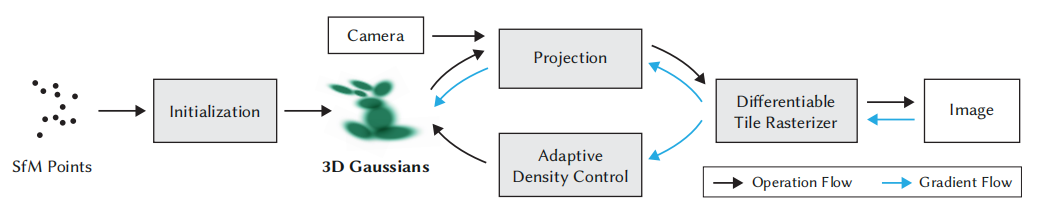
\includegraphics[width=0.95\linewidth]{pipe.png}
\end{center}
\begin{itemize}
    \footnotesize
    \item \textbf{Compact Box} $\to$ tác động tại bước \emph{rasterize} (giảm $\overline{T}$, giảm chi phí render).
    \item \textbf{Multi-view score} $\to$ tác động tại bước \emph{densify/prune} (chọn lọc Gaussian chính xác hơn).
    \item \textbf{Sparse Adam} $\to$ tác động tại bước \emph{optimizer step} (giảm tần suất cập nhật tham số).
\end{itemize}
\end{frame}

% --- Slide 50 ---
\begin{frame}{Tổng kết: từ 3DGS gốc đến FastGS}
\centering
\footnotesize
\begin{tabular}{lll}
\toprule
\textbf{Tham số} & \textbf{3DGS gốc} & \textbf{FastGS} \\
\midrule
\texttt{loss\_thresh} & không có & mới, 0.1 \\
\texttt{grad\_abs\_thresh} & gradient thường & Abs-GS, 0.0012 \\
\texttt{--dense} & cố định & 0.001--0.013 (theo scene extent) \\
\texttt{--highfeature\_lr} & lr chuẩn & 0.005--0.02 (chia thêm /20 trong code) \\
\texttt{--mult} (box multiplier) & 3.0 & 0.5--0.7 \\
\bottomrule
\end{tabular}
\vspace{0.4cm}
\begin{itemize}
    \item FastGS không thay đổi mô hình biểu diễn cảnh, mà tối ưu \textbf{tham số hoá} và \textbf{lịch huấn luyện} dựa trên mô hình chi phí và định luật Amdahl.
    \item Kết quả: tăng tốc đáng kể mà chất lượng tái tạo (PSNR/SSIM) gần như không đổi.
\end{itemize}
\end{frame}
